Il report tecnico NASA CR-2144 \cite{heffley_handling_qualities} contiene i valori delle derivate di stabilità per dieci velivoli. In particolare, nella sezione IX sono riportati i dati relativi al Boeing 747.

\subsubsection*{Selezione delle colonne}

A pagina 229 sono presenti informazioni che permettono di individuare le colonne da utilizzare:

\begin{figure}[H]
    \centering
    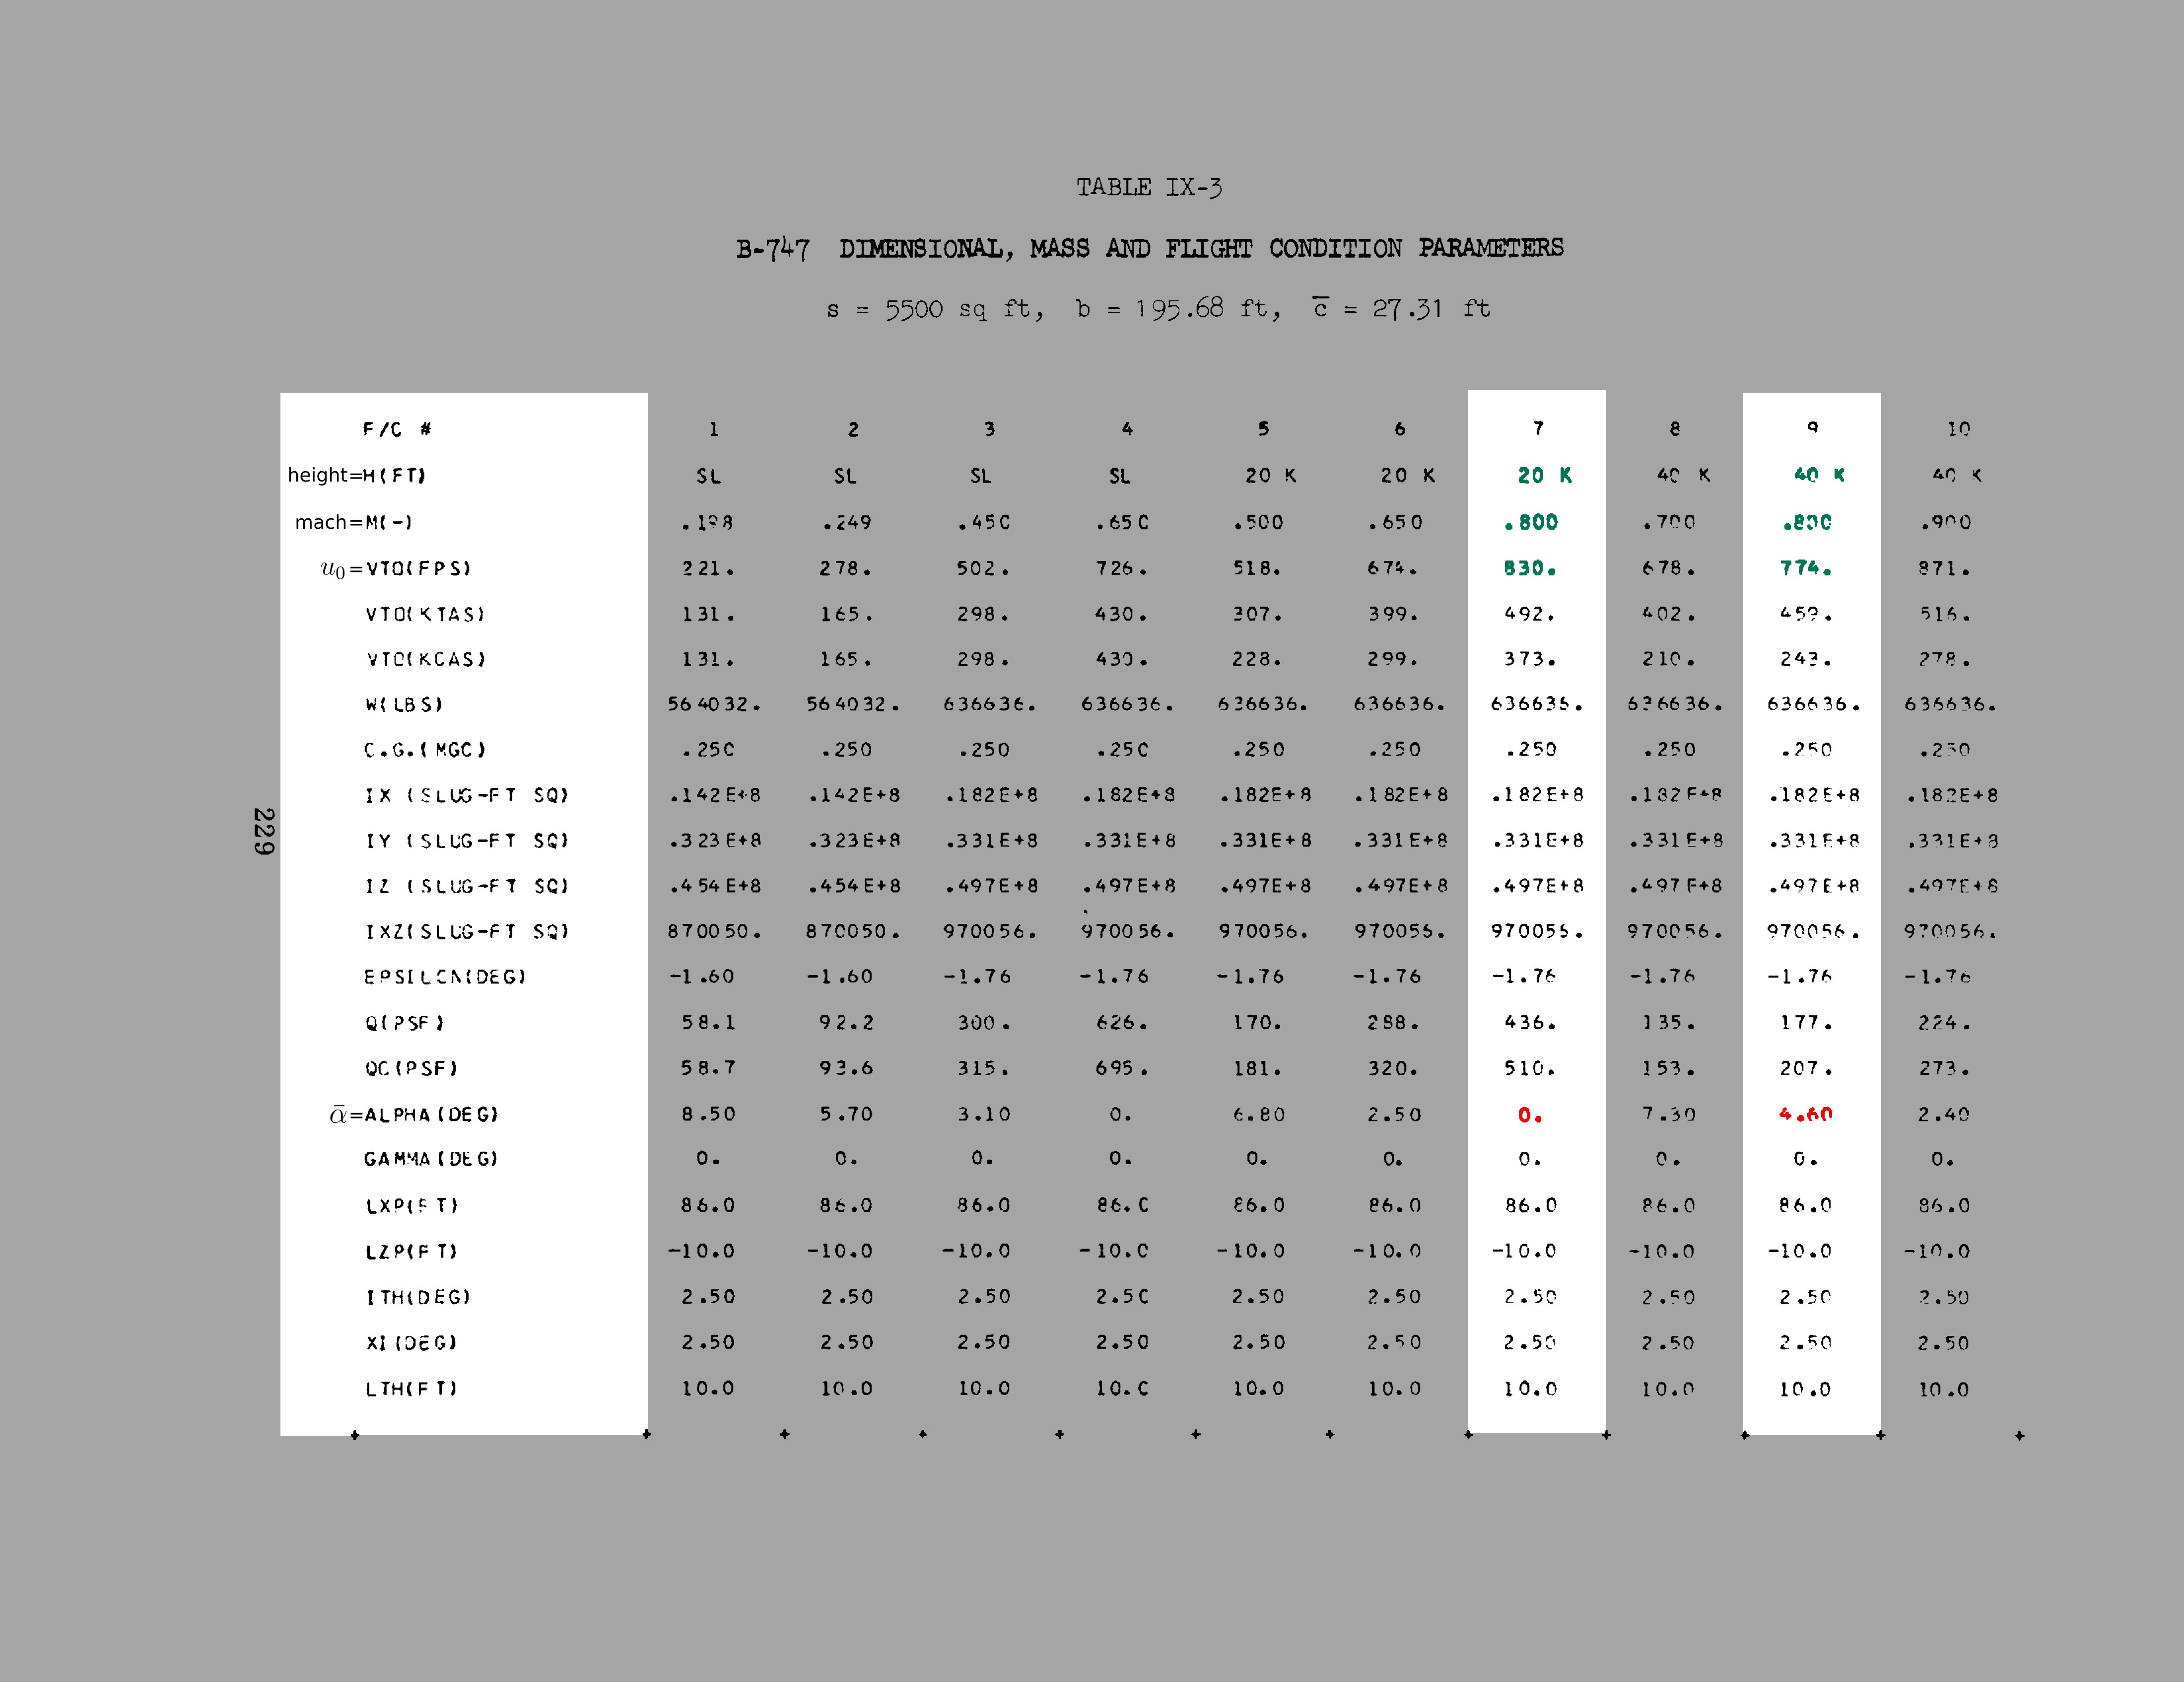
\includegraphics[width=1\linewidth]{Immagini/229.jpg}
\end{figure}

Osservando i valori evidenziati in verde, in particolare l'altitudine e la velocità $u_0$, è possibile selezionare la colonna 7 per le equazioni dei moti longitudinali e la colonna 9 per quelle dei moti laterali.

In questa pagina si può inoltre ricavare il valore di $\bar{\alpha}$, utilizzato in entrambi i set di equazioni.

\subsubsection*{Moti Laterali}

\begin{figure}[H]
    \centering
    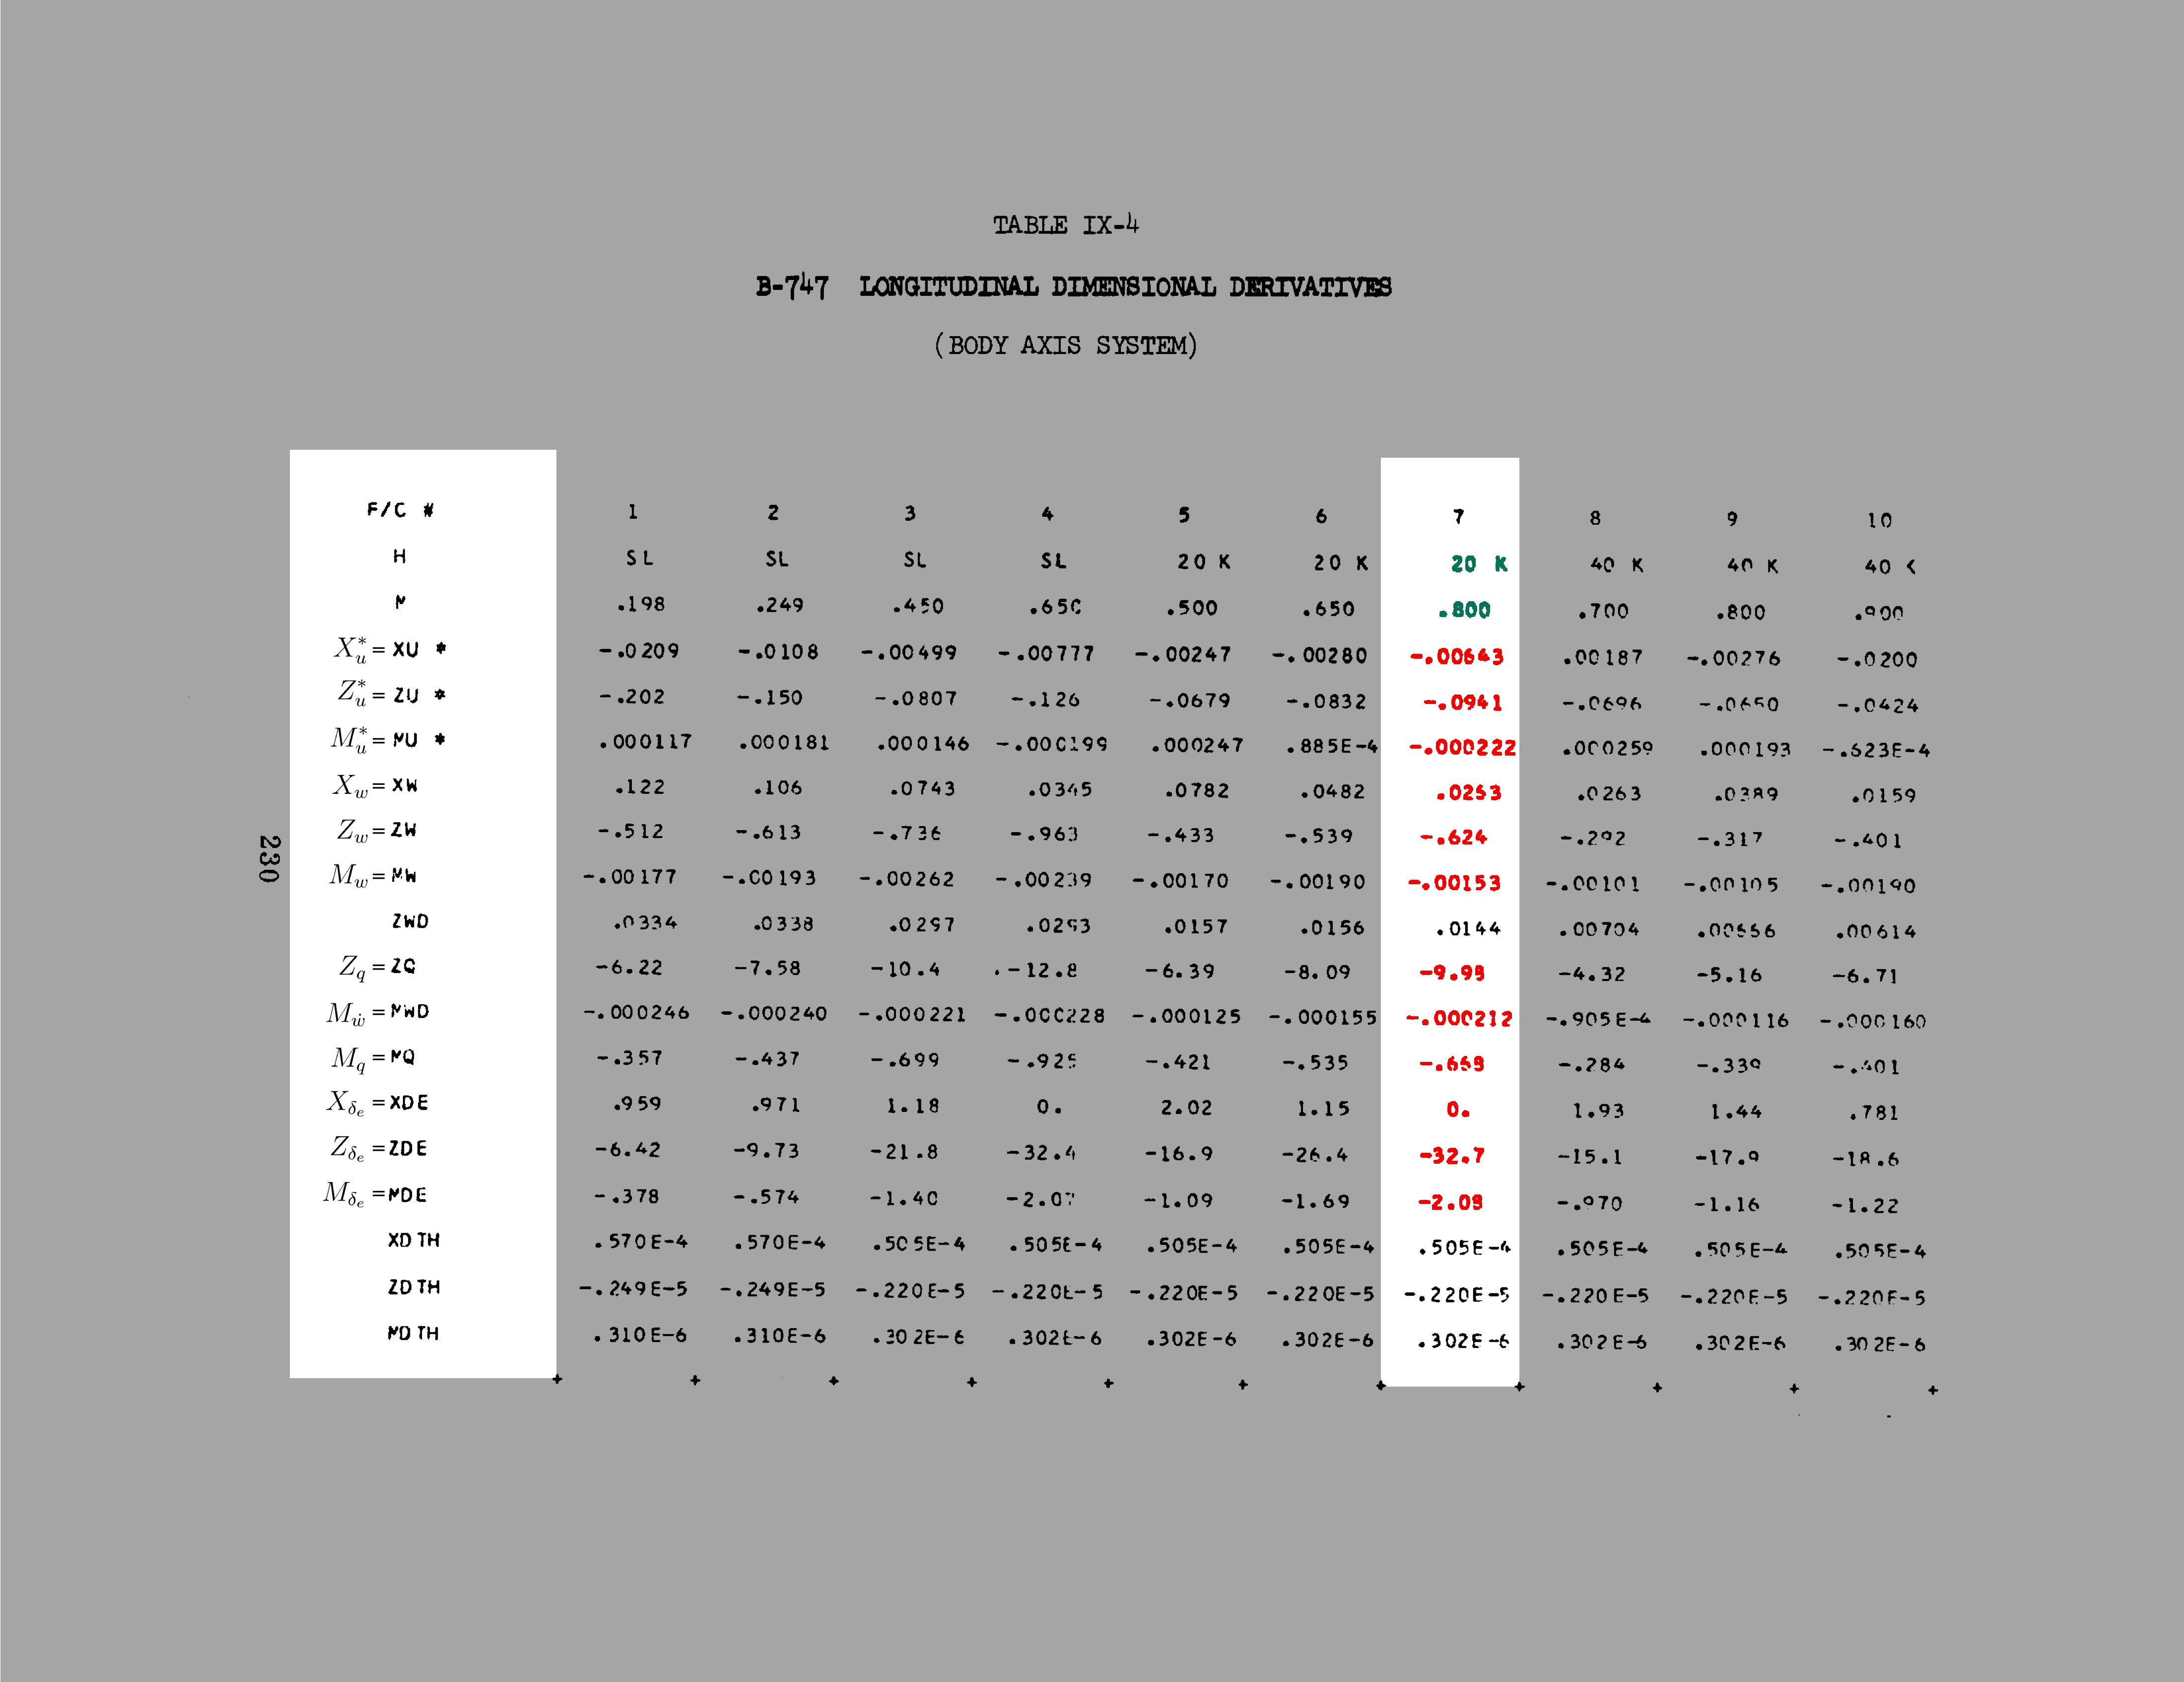
\includegraphics[width=1\linewidth]{Immagini/230.jpg}
\end{figure}

Quasi tutti i valori necessari sono riportati direttamente nella tabella. La traduzione dei simboli è stata possibile grazie alla corrispondenza tra i simboli generati dal computer e la notazione standard, riportata da pagina A-8 a A-10 dell'appendice.

I valori per $M_{(\cdot)}^*$ non sono esplicitamente riportati, ma possono essere ricavati a partire dalle equazioni che li definiscono (vedi \eqref{eq:mStar}), utilizzando i dati presenti nel report.

I termini $T_{\delta_t}\cos\epsilon$, $-T_{\delta_t}\sin\epsilon$ e $M_{\delta_t}^*$ non compaiono in questa tabella, ma possono essere trovati per il Boeing 747 a pagina 40 di \cite{sanches_dynamic_stability_747}.

\subsubsection*{Moti Longitudinali}

\begin{figure}[H]
    \centering
    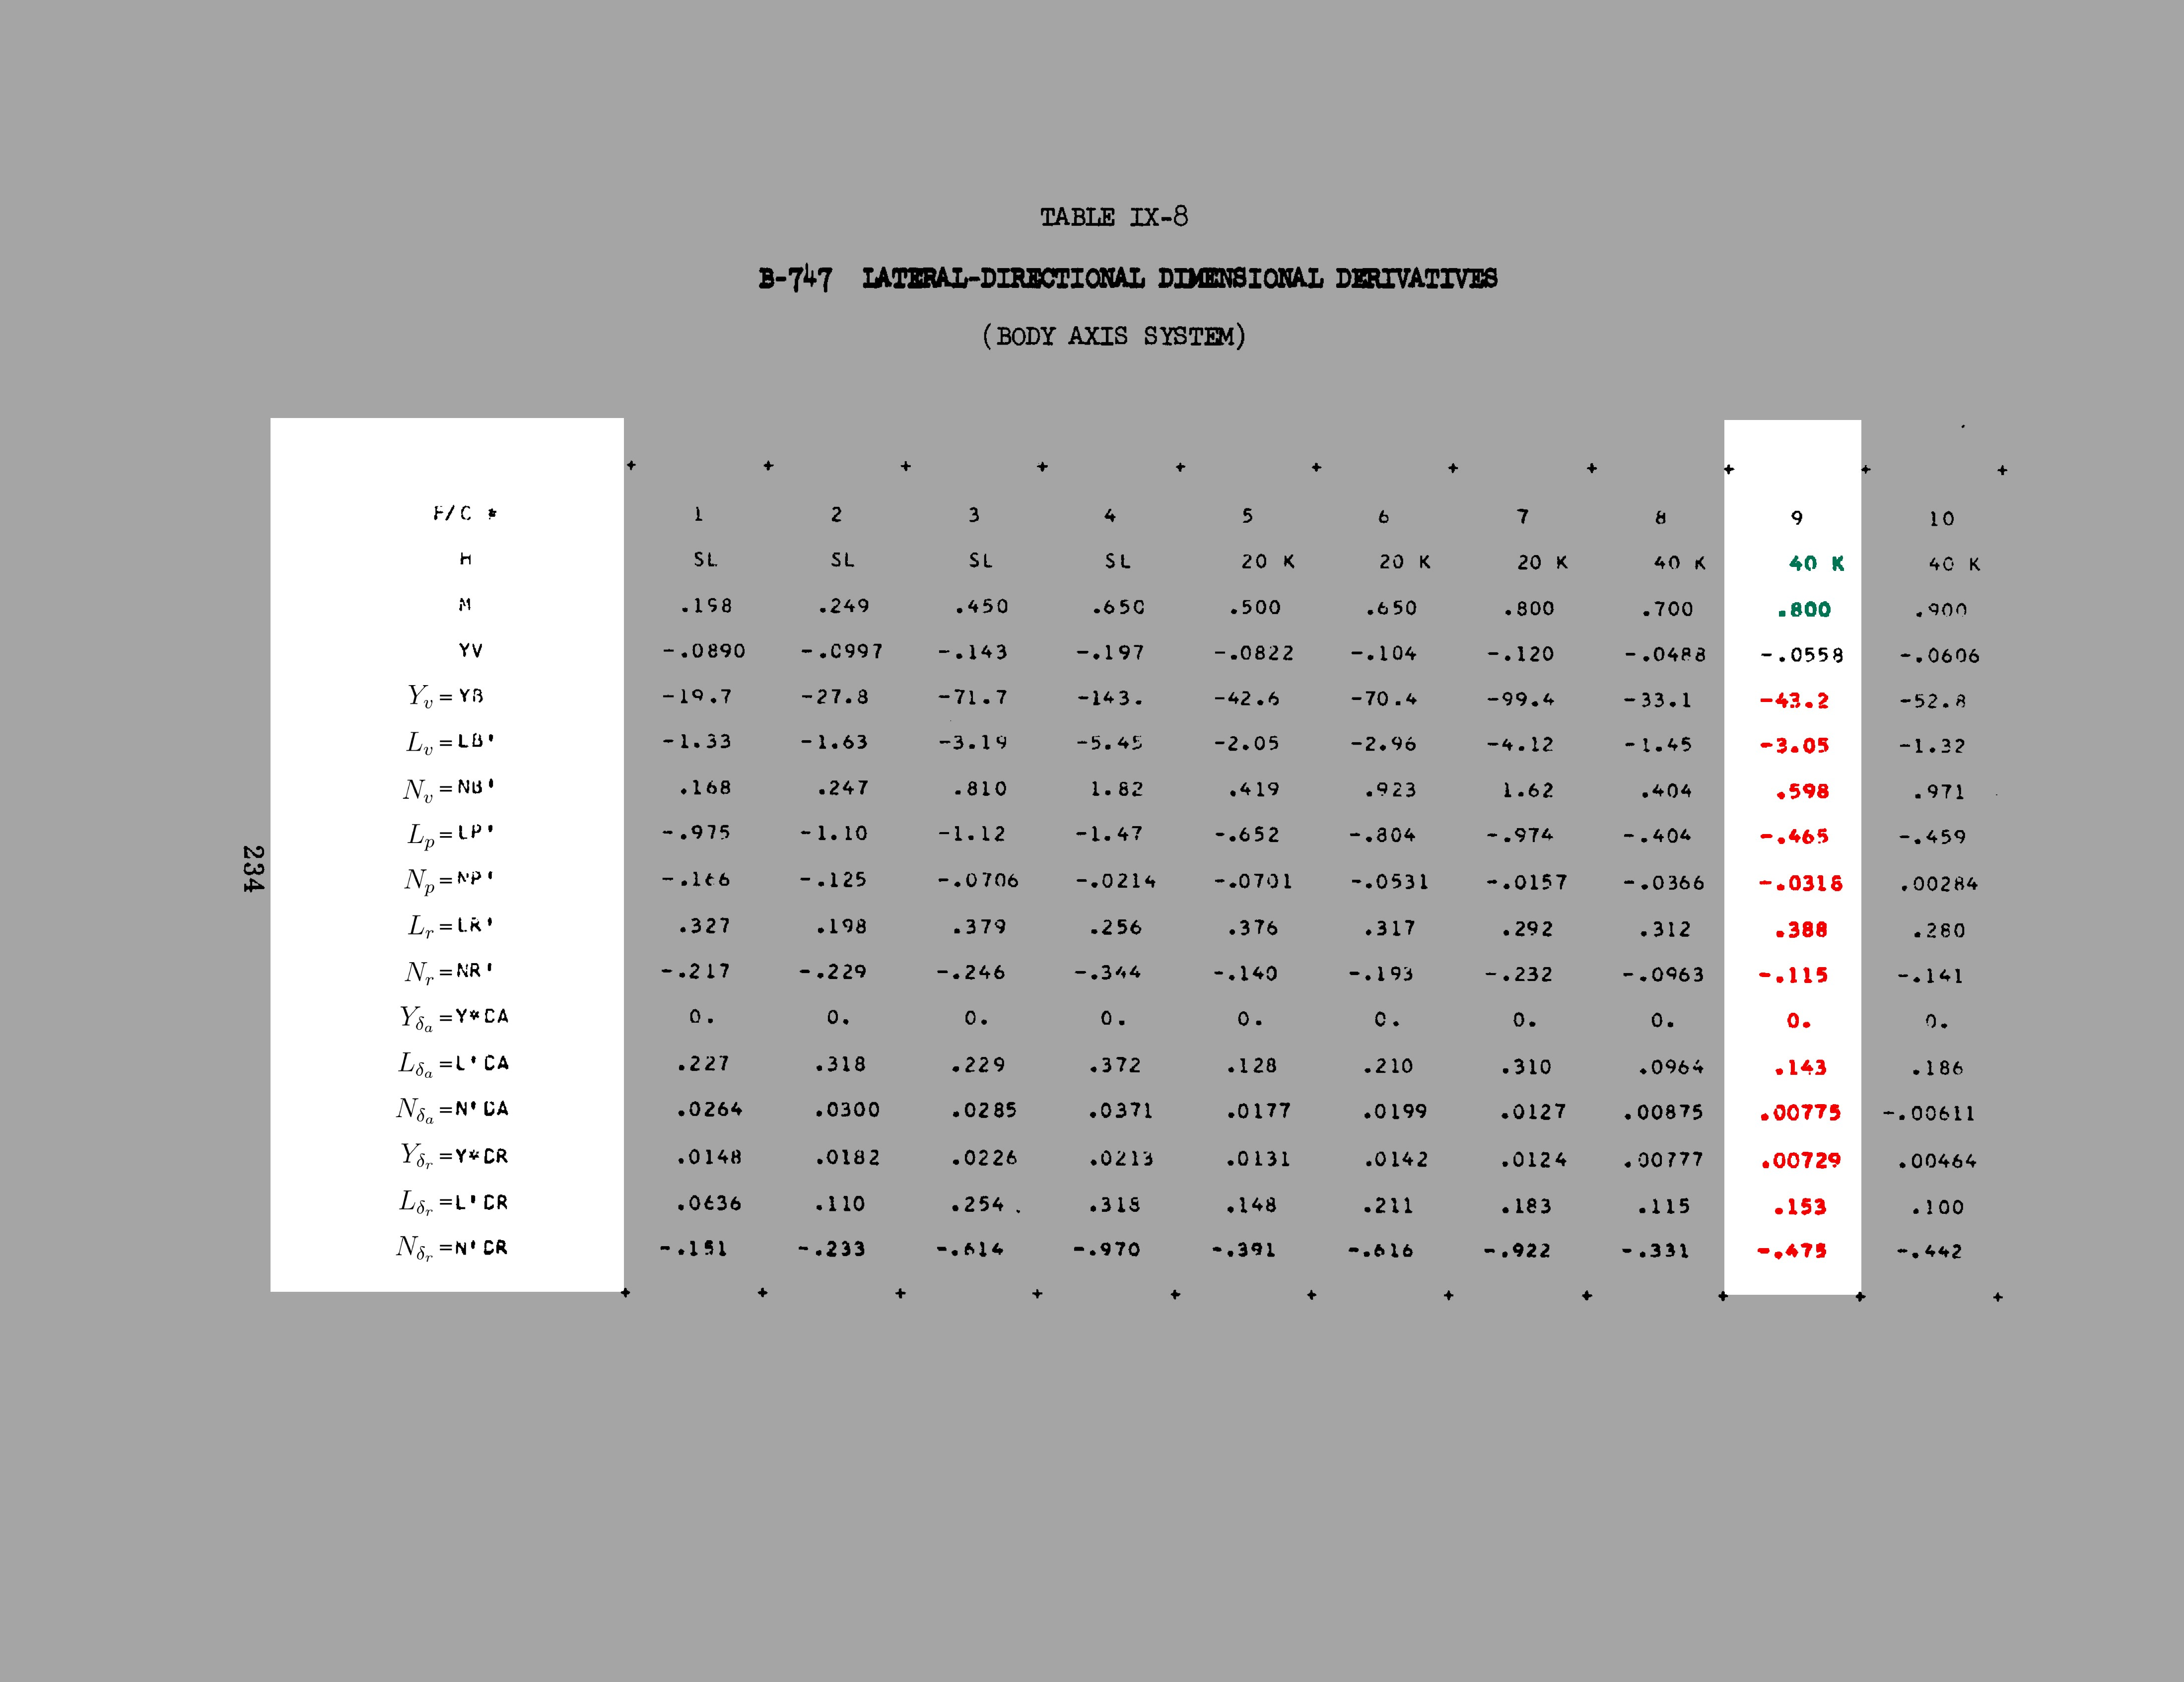
\includegraphics[width=1\linewidth]{Immagini/234.jpg}
\end{figure}

In questo caso la tabella fornisce direttamente tutti i valori necessari per le equazioni dei moti longitudinali, senza bisogno di ulteriori trasformazioni o integrazioni.